% ========================================
% CAPÍTULO 3: METODOLOGÍA, DATOS Y PLAN DE TRABAJO  (criterio 3)
% ========================================

\chapter{METODOLOGÍA, DATOS Y PLAN DE TRABAJO}
\label{ch:metodologia}

\section{Metodología}

Se adapta CRISP-DM a un problema de construcción de un instrumento de medición (Tabla~\ref{tab:etapas}); el diseño sigue la lógica de \emph{design science}: construir un artefacto y evaluarlo contra una verdad conocida \parencite{hevner2004}.

\begin{table}[H]
\centering
\caption{Etapas, propósito y evidencia en el repositorio.}
\label{tab:etapas}
\begingroup\footnotesize\singlespacing
\begin{tabular}{@{}p{3.6cm} p{5.2cm} p{1.2cm} p{5.6cm}@{}}
\toprule
Etapa (CRISP-DM adaptado) & Propósito & Objetivo & Archivo \\
\midrule
Comprensión del problema & Fijar mecanismos de fuga y métrica & OE1 & Capítulo~\ref{ch:introduccion}; \arch{decision_log.md} \\
Comprensión de los datos & Caracterizar los 6 datasets & OE3 & \arch{eda_datasets.py} \\
Preparación & Ruido, faltantes y submuestreo reproducibles & OE3 & \arch{sklearn_loader.py} \\
Modelado (del instrumento) & Generar los 96 pares; construir el auditor & OE2 & \arch{generar_pares_controlados.py}; \arch{03_auditor/} \\
Evaluación & Precisión, recall, VPN, \DOpt{} y pruebas por familia & OE2, OE3 & \arch{run_benchmark.py}; \arch{statistical_analysis.py} \\
Despliegue & Skills y plataforma web & OE4 & \arch{05_skills/}; \arch{06_web/} \\
\bottomrule
\end{tabular}
\endgroup
\end{table}
\donde{VPN: valor predictivo negativo; OE: objetivo específico.}

\section{Datos: origen, obtención y caracterización}
\label{sec:datos}

Se usan seis conjuntos nativos de scikit-learn (Tabla~\ref{tab:datasets}): tres de clasificación (\texttt{breast\_cancer}, \texttt{wine}, \texttt{digits}) y tres de regresión (\texttt{diabetes}, \texttt{california\_housing}, \texttt{make\_friedman1}). Son públicos, no contienen datos personales y se cargan sin copiarlos al repositorio; solo \texttt{california\_housing} se descarga la primera vez. La Figura~\ref{fig:eda} resume la dispersión de escalas y el balance de clases.

\begin{table}[H]
\centering
\caption{Caracterización de los datasets.}
\label{tab:datasets}
\begingroup\footnotesize\singlespacing
\begin{tabular}{@{}l l l r r r r r@{}}
\toprule
ID & Dataset & Tarea & $N$ & Variables & Razón de escalas & Asimetría media & Clase minoritaria \\
\midrule
D1 & breast\_cancer & Clasif. (2) & 569 & 30 & 215.171 & 1,74 & 37,3\,\% \\
D2 & wine & Clasif. (3) & 178 & 13 & 2.530 & 0,43 & 27,0\,\% \\
D3 & digits & Clasif. (10) & 1.797 & 64 & 277 & 4,89 & 9,7\,\% \\
D4 & diabetes & Regresión & 442 & 10 & 1,0 & 0,41 & --- \\
D5 & california\_housing & Regresión & 3.000$^{*}$ & 8 & 1.398 & 10,00 & --- \\
D6 & friedman1 & Regresión & 1.000 & 50 & 1,1 & 0,04 & --- \\
\bottomrule
\end{tabular}
\endgroup
\end{table}
\nota{Razón de escalas: desviación estándar máxima sobre mínima entre variables. $^{*}$Submuestra determinista de 3.000 filas de 20.640 (desviación B1, sección~\ref{sec:desviaciones}). \texttt{digits} tiene 3 columnas constantes.}

\begin{figure}[H]
\centering
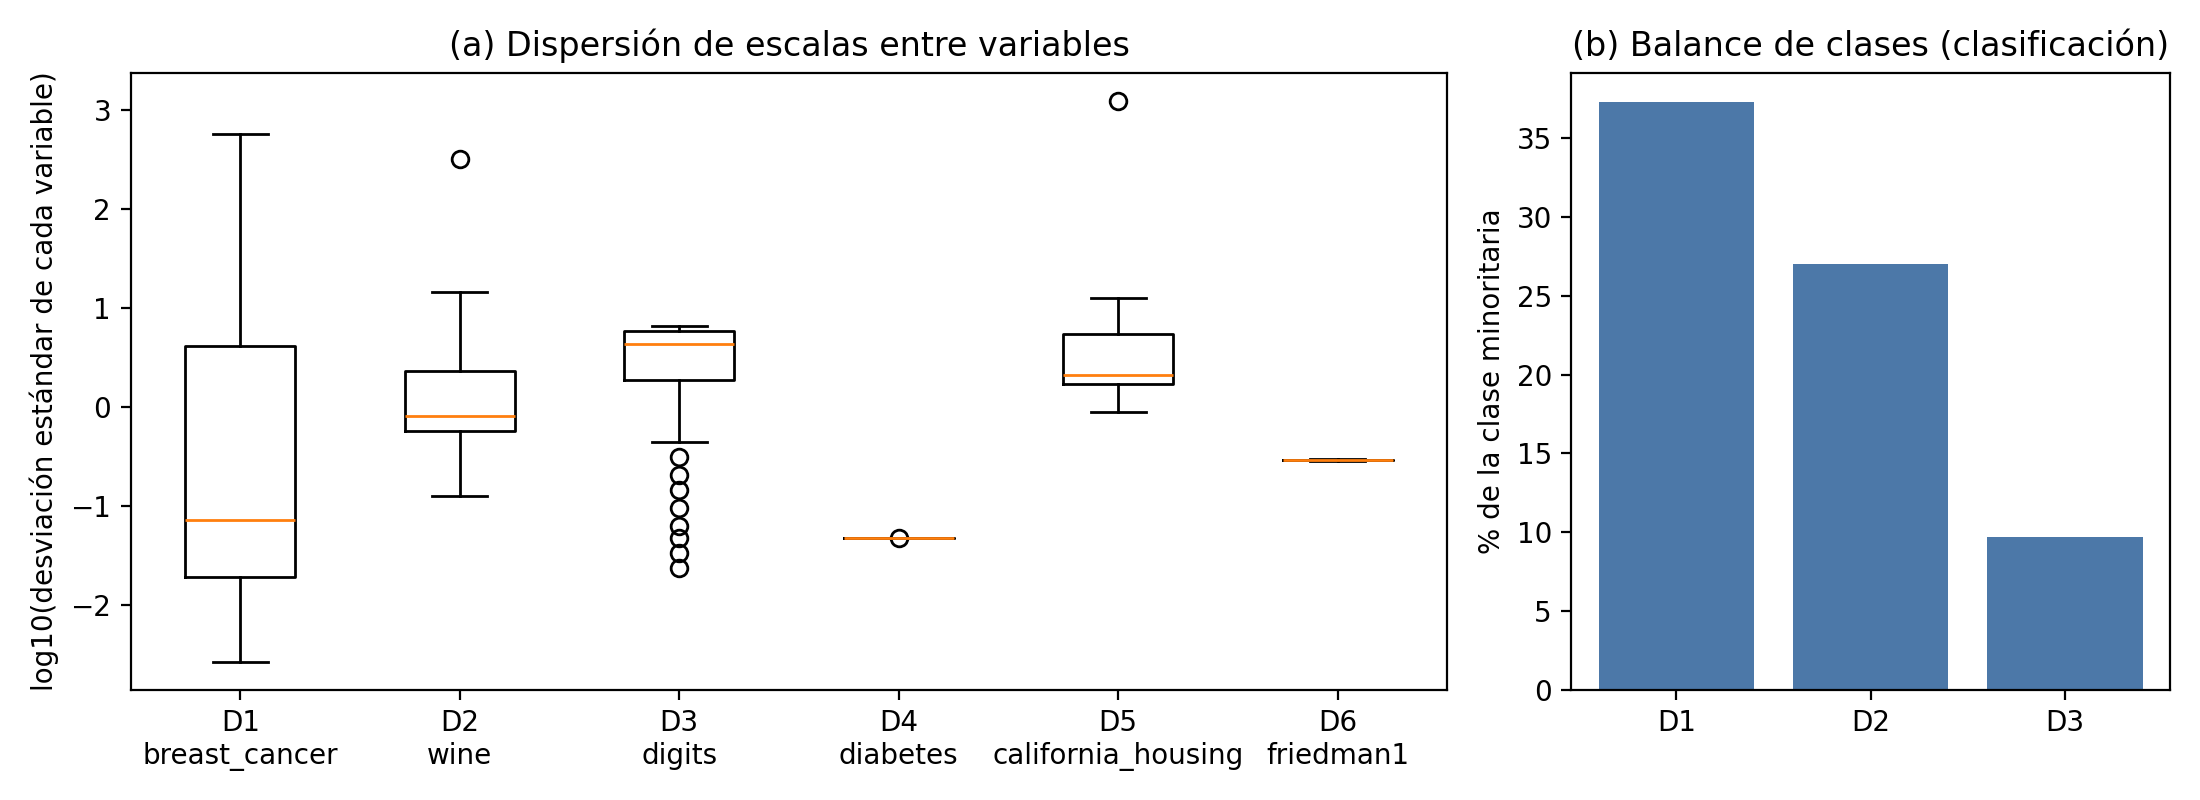
\includegraphics[width=0.95\textwidth]{fig_eda_datasets.png}
\caption{(a) Dispersión de escalas entre variables, en $\log_{10}$ de la desviación estándar. (b) Porcentaje de la clase minoritaria en los datasets de clasificación.}
\label{fig:eda}
\end{figure}

\textbf{Preparación trazable.} (i) \emph{Variante «completo»}: sin faltantes. (ii) \emph{Variante «con\_faltantes»}: se borra el 10\,\% de las celdas con semilla fija (media observada entre 9,8 y 10,1\,\%). (iii) A D1--D5 se les agregan 50 columnas de ruido gaussiano, porque la fuga por selección solo se manifiesta si hay variables inútiles entre las cuales elegir; D6 ya trae 45. Todo usa la semilla 42, y dos ejecuciones producen datos idénticos (verificado en las pruebas automáticas).

\textbf{Representatividad y limitaciones.} Son datasets clásicos, limpios, pequeños y tabulares; no representan datos reales ruidosos, de gran escala ni con estructura temporal o jerárquica, y los LLM probablemente los vieron durante su entrenamiento. Por la dispersión de escalas (Figura~\ref{fig:eda}a), el escalado debería afectar sobre todo a los modelos sensibles a la escala; por la asimetría de D5 (10,0) se esperan valores atípicos que desestabilicen a la red neuronal, y así ocurrió (sección~\ref{sec:desviaciones}). Con ROC-AUC cercana a 1 en D1--D3 hay un efecto techo que limita cuánto optimismo puede observarse en clasificación.

\section{Diseño experimental}
\label{sec:diseno}

Para cada combinación de 6 datasets $\times$ 4 familias $\times$ 4 tipos de fuga, un generador escribe un script con fuga (\texttt{leaky}) y otro idéntico sin ella (\texttt{clean}): \textbf{96 pares, 192 scripts}. Los modelos son \texttt{RandomForest}, \texttt{HistGradientBoosting}, \texttt{LogisticRegression} o \texttt{Ridge}, y \texttt{MLPClassifier} o \texttt{MLPRegressor}. Como la verdad se conoce por construcción, no se necesitan anotadores.

Cada script se audita con \textbf{dos mecanismos independientes}. El primero es un análisis del árbol sintáctico (\texttt{ast}) con tres reglas: \emph{R-Split} (ajuste antes de \texttt{train\_test\_split}), \emph{R-CV} (ajuste fuera de un \texttt{Pipeline} cuyo resultado entra a la validación cruzada) y \emph{R-Test} (ajuste con una variable que parece de prueba). El segundo es un verificador en ejecución que cuenta con cuántas filas se ajusta cada transformador y declara fuga si coincide con el total del dataset. El detector híbrido declara fuga si cualquiera de los dos la ve. El auditor nunca consulta a un LLM; los LLM serán solo los sujetos de estudio que generan los pipelines en Capstone~II.

\section{Plan de trabajo actualizado y desviaciones}
\label{sec:desviaciones}

\begin{table}[H]
\centering
\caption{Plan de trabajo (estado a octubre de 2026).}
\label{tab:plan}
\begingroup\footnotesize\singlespacing
\begin{tabular}{@{}p{3.0cm} p{10.4cm} p{2.0cm}@{}}
\toprule
Periodo & Actividad & Estado \\
\midrule
Capstone I & Reformulación del problema y la métrica; datasets; banco de 96 pares; auditor AST y runtime; refactorizador; benchmark y \DOpt; Skills y plataforma web (prototipo); informe & Hecho \\
Capstone II, sem. 1--4 & Generar pipelines con 6--8 LLM reales (24 tareas por modelo) y auditarlos; ejecutarlos en un entorno aislado & Pendiente \\
Capstone II, sem. 5--8 & Mejorar el auditor (alias de importación, funciones auxiliares, \texttt{ColumnTransformer}); ampliar la evaluación independiente de 13 a $\geq 60$ scripts & Pendiente \\
Capstone II, sem. 9--12 & Más datasets con señal débil; intervalos bootstrap por dataset; piloto de uso con 3--5 personas & Pendiente \\
Capstone II, sem. 13--16 & Redacción de la tesis y defensa & Pendiente \\
\bottomrule
\end{tabular}
\endgroup
\end{table}

\textbf{Desviaciones respecto del plan original} (justificación completa en \arch{07_informe/decision_log.md}):
\begin{itemize}
  \item \textbf{B1.} \texttt{california\_housing} se submuestrea a 3.000 filas: \texttt{KNNImputer} crece con $n^2$ y el banco de 192 scripts no sería ejecutable en un portátil.
  \item \textbf{B2.} El sobremuestreo (SMOTE) no se mide, porque no pertenece a scikit-learn; el cuarto tipo es «combinada».
  \item \textbf{B3.} \texttt{LogisticRegression} usa \texttt{max\_iter=2000} para evitar avisos de no convergencia.
  \item \textbf{C1.} En una primera corrida, los modelos lineal y MLP se evaluaban sin escalar en las fugas de imputación y selección, lo que producía diferencias negativas por inestabilidad numérica (hasta $-0{,}155$ en \texttt{wine}). Se corrigió añadiendo un escalador interno idéntico en ambas versiones; los resultados descartados se conservan en \arch{results/corrida1_descartada/}.
  \item \textbf{C2.} Un \texttt{MLPRegressor} divergió en un pliegue ($R^2=-21$ en \texttt{california\_housing}; promedio $-3{,}86$). Se definió, \textbf{después de ver el problema}, que un par es degenerado si algún pliegue tiene $R^2<-1$; se excluyó 1 par de 96 y se lista aparte.
\end{itemize}
